\documentclass[conference]{IEEEtran}
\IEEEoverridecommandlockouts

\usepackage{cite}
\usepackage{amsmath,amssymb,amsfonts}
\usepackage{graphicx}
\usepackage{textcomp}
\usepackage{xcolor}
\usepackage{booktabs}
\usepackage{multirow}
\usepackage{array}
\usepackage{url}

\setlength{\textfloatsep}{8pt plus 1pt minus 2pt}
\setlength{\floatsep}{7pt plus 1pt minus 2pt}
\setlength{\intextsep}{7pt plus 1pt minus 2pt}

\newcommand{\method}{TShape-Zero+}
\newcommand{\direct}{TShape-Zero}
\newcommand{\pfone}{Point-F1}
\newcommand{\efone}{Event-F1}
\newcommand{\DirectMacroPoint}{0.802}
\newcommand{\DirectMacroEvent}{0.701}
\newcommand{\PatternMacroPoint}{0.802}
\newcommand{\PatternMacroEvent}{0.701}
\newcommand{\FinalMacroPoint}{0.846}
\newcommand{\FinalMacroEvent}{0.733}
\newcommand{\GuardMacroPoint}{0.846}
\newcommand{\GuardMacroEvent}{0.726}
\newcommand{\PatternTrainLossInitial}{0.090}
\newcommand{\PatternTrainLossFinal}{0.024}
\newcommand{\PatternTrainEpochs}{30.000}
\newcommand{\DirectAIOPSPoint}{0.867}
\newcommand{\DirectAIOPSEvent}{0.758}
\newcommand{\FinalAIOPSPoint}{0.895}
\newcommand{\FinalAIOPSEvent}{0.769}
\newcommand{\DirectNABPoint}{0.999}
\newcommand{\DirectNABEvent}{0.926}
\newcommand{\FinalNABPoint}{0.999}
\newcommand{\FinalNABEvent}{0.918}
\newcommand{\DirectTODSPoint}{0.694}
\newcommand{\DirectTODSEvent}{0.622}
\newcommand{\FinalTODSPoint}{0.766}
\newcommand{\FinalTODSEvent}{0.673}
\newcommand{\DirectUCRPoint}{0.637}
\newcommand{\DirectUCREvent}{0.380}
\newcommand{\FinalUCRPoint}{0.669}
\newcommand{\FinalUCREvent}{0.396}
\newcommand{\DirectWSDPoint}{0.951}
\newcommand{\DirectWSDEvent}{0.869}
\newcommand{\FinalWSDPoint}{0.967}
\newcommand{\FinalWSDEvent}{0.873}
\newcommand{\DirectYahooPoint}{0.666}
\newcommand{\DirectYahooEvent}{0.651}
\newcommand{\FinalYahooPoint}{0.779}
\newcommand{\FinalYahooEvent}{0.769}


\def\BibTeX{{\rm B\kern-.05em{\sc i\kern-.025em b}\kern-.08em
    T\kern-.1667em\lower.7ex\hbox{E}\kern-.125emX}}

\begin{document}

\title{\method: An Out-of-the-Box TShape for Zero-Shot KPI Anomaly Detection}

\author{
    \IEEEauthorblockN{
        Hang Cui\IEEEauthorrefmark{1}\IEEEauthorrefmark{2},
        Jingjing Li\IEEEauthorrefmark{1},
        Haotian Si\IEEEauthorrefmark{1}\IEEEauthorrefmark{2},
        Quan Zhou\IEEEauthorrefmark{1}\IEEEauthorrefmark{2},
        Changhua Pei\IEEEauthorrefmark{1}\IEEEauthorrefmark{3},
        Gaogang Xie\IEEEauthorrefmark{1},
        Dan Pei\IEEEauthorrefmark{4}
    }
    \IEEEauthorblockA{\IEEEauthorrefmark{1}Computer Network Information Center, Chinese Academy of Sciences\\
    \{cuihang, ljj, htsi, zhouquan, chpei, xie\}@cnic.cn}
    \IEEEauthorblockA{\IEEEauthorrefmark{2}University of the Chinese Academy of Sciences}
    \IEEEauthorblockA{\IEEEauthorrefmark{3}Hangzhou Institute for Advanced Study, University of Chinese Academy of Sciences}
    \IEEEauthorblockA{\IEEEauthorrefmark{4}Tsinghua University, peidan@tsinghua.edu.cn}
}

\maketitle

\begin{abstract}
KPI anomaly detection is a first line of defense for software reliability, but a new service rarely has incident labels or time for per-metric model training. TShape is effective in its original target-trained setting. We ask a constructive artifact-engineering question: how can TShape become one reusable detector that scores an unseen KPI without benchmark-domain weight updates? We first reproduce the original effect and stress-test direct reuse under the same EasyTSAD metrics. We then propose \method{}, whose single 0.138-MiB checkpoint is trained only on a Pattern Bank of generated temporal dynamics and random context incidents. At inference, an open-box Residual Guard combines the neural shape residual with rolling-median, spectral, and robust-deviation evidence. We evaluate one frozen checkpoint on all 834 series from six industrial or public monitoring datasets (15.1 million observations), using one fixed seed and no target-label model selection. A broad ledger includes three focal official forecasting-foundation checkpoints, every baseline family in the original TShape study, source-adaptation diagnostics, and no-training controls. Pattern pretraining alone obtains macro \pfone{}/\efone{} of \DirectMacroPoint{}/\DirectMacroEvent{}; the guarded product obtains \FinalMacroPoint{}/\FinalMacroEvent{}, exceeding the three focal frozen checkpoints while preserving channel attribution. Full-size, weight, normalization, and paired-series ablations state where the neural channel helps and where the guard supplies the reliability floor. We release the model, verification ledger, CLI, and a web scorer that converts an uploaded KPI history into aligned anomaly scores and ranked suspicious points.
\end{abstract}

\begin{IEEEkeywords}
time-series anomaly detection, replication, negative results, zero-shot learning, software reliability
\end{IEEEkeywords}

\section{Introduction}

\begin{figure}[t]
  \centering
  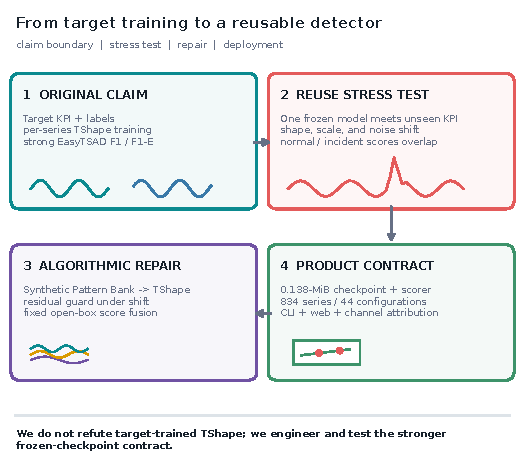
\includegraphics[width=\columnwidth]{figures/fig_intro_strict.pdf}
  \caption{From target-trained TShape to one out-of-the-box detector. We preserve the original claim, stress-test direct artifact reuse, repair temporal coverage with a synthetic Pattern Bank, and guard shifted KPIs with inspectable residual evidence.}
  \label{fig:intro}
\end{figure}

Modern software systems expose thousands of key performance indicators (KPIs), including latency, throughput, error rate, queue depth, CPU utilization, cache hit rate, and service-specific counters. Their anomaly detectors often fire before root-cause localization, incident response, rollback, or capacity control. Consequently, the detector is not an isolated machine-learning component: it is part of the operational reliability boundary. Missing an incident delays mitigation, while an unstable score stream overwhelms on-call engineers.

This boundary is difficult to maintain for newly deployed services. Labels are scarce, incident distributions change after releases, and training a model for every metric is expensive at fleet scale. Industrial TSAD benchmarks report large differences across datasets, protocols, and deployment assumptions~\cite{si2024timeseriesbench,liu2024elephant,paparrizos2022tsb}. Practitioners therefore have a concrete reason to prefer a reusable checkpoint that can score an unseen KPI immediately. Recent forecasting foundation models reinforce this checkpoint-reuse expectation by advertising cross-series inference through a common prediction interface~\cite{liu2024timer,ansari2024chronos,das2024timesfm,liu2025sundial,shi2024timemoe}.

TShape targets complex shapelet anomalies with convolutional patch encoding and local/global attention~\cite{cui2025tshape}. Its original paper trains on each target environment and reports strong EasyTSAD F1 and event-weighted F1. We neither dispute nor retroactively enlarge that claim. Instead, we study a realistic product requirement encouraged by checkpoint-oriented time-series systems: ship one trained model, accept an unseen KPI history, and immediately return useful anomaly scores. This paper is therefore an \emph{artifact reuse stress test plus repair protocol}, not a refutation of a zero-shot claim made by the original work.

The first stress test confirms why a model class is not yet a product contract. A next-step residual can execute on any sequence, but a target-trained checkpoint has learned target-specific local shapes, patch relations, and residual scale. Under a shifted KPI, routine variation can outrank incidents. Missing checkpoints, preprocessing metadata, a scoring command, resource evidence, and failure documentation compound this model-level risk. We convert those observations into three design challenges.

\textbf{Challenge 1: open-world temporal diversity.}
KPI histories combine flat regions, trends, cycles, staircases, random walks, bursts, variance changes, and recoveries. A model trained on one operational environment cannot enumerate this space. Our Pattern Bank samples 20 temporal generators under randomized amplitude, offset, phase, slope, reversal, and noise, then injects context-only incidents while keeping the next-value target clean. This creates a benchmark-independent pretraining distribution rather than a hidden mixture of the six evaluation datasets.

\textbf{Challenge 2: distribution shift.}
An unseen service can differ in scale, noise, seasonality, and smoothness. \method{} adds a Residual Guard made of rolling-median, spectral-residual, and rolling-MAD channels. A fixed reliability budget reserves 85\% of the fused score for these transparent controls and 15\% for TShape. Each channel remains observable, making the repair falsifiable rather than hiding a strong residual baseline inside a new model name.

\textbf{Challenge 3: executable artifact readiness.}
A reusable detector is more than weights. It needs a preprocessing contract, score alignment, coverage checks, immutable metadata, resource evidence, a callable interface, and documented boundaries. Our CLI and web service invoke the same scorer and return the input trace, fused score, neural score, guard score, and top-$k$ indices. EasyTSAD's label-informed best threshold remains evaluation-only.

Fig.~\ref{fig:intro} summarizes this transition. The contributions are:
\begin{itemize}
    \item \textbf{Replication and industrial reuse stress test.} We preserve the original target-trained claim, replay and complete its EasyTSAD evidence, and evaluate the stronger out-of-the-box requirement with explicit data-access contracts.
    \item \textbf{The \method{} algorithmic upgrade.} We introduce benchmark-independent Pattern Bank pretraining and a residual-first guard with open-box channel attribution. Nested bank-size, normalization, pairwise-channel, and fusion-weight ablations isolate what is learned, what is guarded, and why.
    \item \textbf{Full evidence and executable deployment.} One seed and one frozen checkpoint score all 834 series. We compare 44 configurations, publish paired uncertainty and resource evidence, and release the model, code, and interactive scorer at \url{https://github.com/CSTCloudOps/TShape-Zero}.
\end{itemize}

\section{Preliminaries and Motivation}

\subsection{Time-Series Anomaly Detection}

Let a univariate KPI be $x_{1:T}\in\mathbb{R}^{T}$, with labels $y_t\in\{0,1\}$ available only to retrospective evaluation. A detector returns scores $s_t\in\mathbb{R}$, where a larger value means more anomalous. A threshold $\tau$ induces $\hat y_t(\tau)=\mathbb{1}[s_t\geq\tau]$. An anomaly event $e=[a,b]$ is a maximal contiguous interval of positive labels, with length $L_e=b-a+1$ and event score $m_e=\max_{t\in e}s_t$.

\textbf{One EasyTSAD protocol throughout.}
The paper reports only the two metrics used by TShape's EasyTSAD evaluation. \texttt{PointF1PA()} replaces every event by the weighted item $(m_e,L_e,1)$ and every normal point by $(s_t,1,0)$. \texttt{EventF1PA(mode="log")} instead gives an event weight
\begin{equation}
  w_e=\left\lfloor \log_3(L_e+3)\right\rfloor,
  \label{eq:event-weight}
\end{equation}
while a normal point retains unit weight. Each implementation sorts these weighted items by score, sweeps every candidate threshold, and reports the maximum harmonic mean of precision and recall. We call the outputs \pfone{} (F1) and \efone{} (F1-E), respectively. We macro-average valid series and report the number of all-normal series separately.

This definition matters for interpretation. The threshold is selected using labels, so these metrics assess score separability under the original TShape protocol; they are not deployable automatic calibration rules. Point adjustment can also make long events easier to detect~\cite{kim2022rigorous}. We retain it because the original TShape claim uses this protocol, apply the same implementation to every score stream, and avoid mixing it with unrelated ranking or threshold metrics.

\subsection{What ``Out of the Box'' Means}

For target dataset $D_q$, a target-trained model estimates $\theta_q$ from $D_q^{\mathrm{train}}$. An out-of-the-box model instead ships one immutable parameter set $\theta^\star$ before $D_q$ is opened:
\begin{equation}
 \theta^\star \perp
 \left(D_q^{\mathrm{train}},D_q^{\mathrm{test}},Y_q\right),
 \qquad
 s_q=\mathcal{S}_{\theta^\star}\!\left(x_q;\mathcal{P}_q\right).
 \label{eq:zero-contract}
\end{equation}
Here $\perp$ means that no benchmark value, label, or gradient is used to fit or choose $\theta^\star$; $\mathcal{P}_q$ may use unlabeled target history for affine scaling. This is \emph{frozen-model zero-shot scoring with unlabeled context}, not a setting with no access to the sequence being scored. The same checkpoint must serve AIOPS, NAB, TODS, UCR, WSD, Yahoo, and a future unknown KPI.

An out-of-the-box artifact is the tuple
\begin{equation}
 \mathcal{A}=(\theta,\mathcal{P},\mathcal{S},\mathcal{I},\mathcal{V},\mathcal{F}),
 \label{eq:artifact}
\end{equation}
where $\mathcal{P}$ is preprocessing, $\mathcal{S}$ scoring, $\mathcal{I}$ an inference interface, $\mathcal{V}$ executable verification, and $\mathcal{F}$ a failure card. This artifact contract connects model reuse with software release engineering and complements model cards and dataset documentation~\cite{mitchell2019modelcards,gebru2021datasheets}.

\subsection{TShape and the Reuse Gap}

\begin{figure}[t]
  \centering
  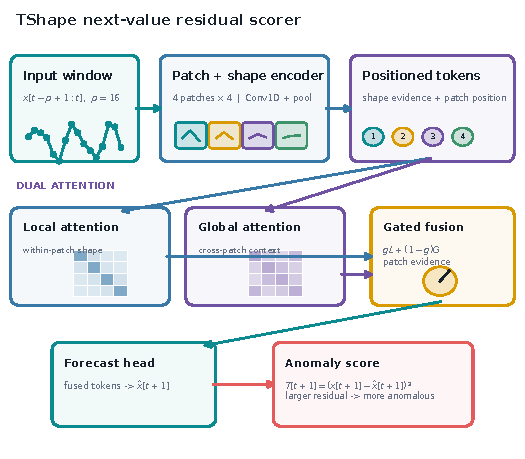
\includegraphics[width=\columnwidth]{figures/fig_tshape_architecture_strict.pdf}
  \caption{TShape next-step residual scorer. A $p=16$ history is split into four patches; convolutional shape tokens feed local and global attention, gated fusion, and a forecasting head. The squared next-value error is the anomaly score.}
  \label{fig:tshape}
\end{figure}

TShape maps the history $w_t=x_{t-p+1:t}$ to a next-value prediction and emits
\begin{equation}
  T_{t+1}=\left(x_{t+1}-f_{\theta}(w_t)\right)^2.
  \label{eq:tshape-score}
\end{equation}
As Fig.~\ref{fig:tshape} shows, convolutional patch encoders model short shapes, local attention models within-patch dependence, global attention connects nonadjacent patches, and a learned gate fuses both views. This interface makes checkpoint reuse technically easy: the same tensor shape produces a residual on a new KPI. It does not ensure that source-learned attention or residual scale transfers.

\begin{figure}[t]
  \centering
  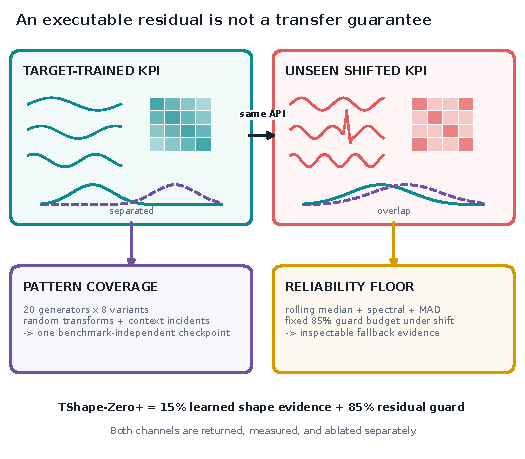
\includegraphics[width=\columnwidth]{figures/fig_motivation_strict.pdf}
  \caption{Why an executable residual interface is not a transfer guarantee. A frozen predictor can preserve its API while shifted shapes alter attention and make normal and anomalous residuals overlap. Pattern pretraining broadens shape exposure; the Residual Guard supplies an inspectable fallback.}
  \label{fig:motivation}
\end{figure}

Fig.~\ref{fig:motivation} illustrates the failure mode. The original target-trained model sees the target's scale and recurring patterns. A universal checkpoint sees a generated training distribution $P_{\mathrm{PB}}$, while an unseen KPI follows $P_q$; generally
\begin{equation}
 P_q(w_t,x_{t+1})\neq P_{\mathrm{PB}}(w_t,x_{t+1}).
 \label{eq:shift}
\end{equation}
The code continues to run, while anomaly-score ordering changes. This distinction is precisely what a reuse stress test should expose.

\begin{figure}[t]
  \centering
  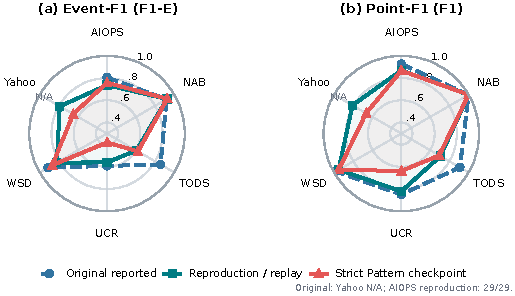
\includegraphics[width=\columnwidth]{figures/fig03_easytsad_protocol_radar.pdf}
  \caption{Protocol-separated TShape evidence. The original paper reports five target-trained datasets; reproduction combines immutable score replay with faithful completion; Strict Zero evaluates one synthetic-only Pattern checkpoint unchanged on all six datasets. Yahoo is an artifact extension.}
  \label{fig:radar}
\end{figure}

The radar view in Fig.~\ref{fig:radar} prevents a misleading one-number comparison. It shows (i) the five values reported by the original paper, (ii) a provenance-preserving six-dataset reproduction from stored replay plus faithful re-execution, and (iii) the single Pattern-only checkpoint before guarding. The polygons describe different claims and are never subtracted as if their training scopes were identical.

\begin{table}[t]
\caption{Claim-separated TShape evidence under the two EasyTSAD metrics. Cells are Point-F1 / Event-F1. Original values are transcribed; reproduction combines stored-score replay and protocol-faithful completion; Strict Zero is one synthetic-only Pattern checkpoint evaluated unchanged on every dataset.}
\label{tab:tshape-claim-boundary}
\centering
\scriptsize
\setlength{\tabcolsep}{3.0pt}
\begin{tabular}{lccc}
\toprule
Dataset & Original reported & Reproduction & Strict Zero \\
\midrule
AIOPS & 0.926 / 0.805 & 0.869 / 0.736 & 0.867 / 0.758 \\
NAB & 0.998 / 0.919 & 0.998 / 0.923 & 0.999 / 0.926 \\
TODS & 0.908 / 0.856 & 0.706 / 0.605 & 0.694 / 0.622 \\
UCR & 0.849 / 0.592 & 0.819 / 0.560 & 0.637 / 0.380 \\
WSD & 0.983 / 0.914 & 0.953 / 0.822 & 0.951 / 0.869 \\
Yahoo & -- & 0.808 / 0.791 & 0.666 / 0.651 \\
\bottomrule
\end{tabular}
\end{table}


The reproduction restores the original target-trained comparison without borrowing it as zero-shot evidence. Stored scores are replayed when complete; missing AIOPS scores are completed with the original per-series recipe; TODS is re-executed against the packaged labels. Yahoo has no original-paper cell and is marked as an extension. In contrast, the Strict Zero column uses one synthetic-only checkpoint unchanged on all six targets. This separation explains why a lower strict score can motivate a repair without contradicting TShape's published in-distribution claim.

\begin{table}[t]
\caption{Target-context harness diagnostic (Point-F1 / Event-F1). These three-epoch variants test preprocessing and window sensitivity; they are not zero-shot competitors.}
\label{tab:harness-diagnostic}
\centering
\scriptsize
\setlength{\tabcolsep}{2.5pt}
\begin{tabular}{lccc}
\toprule
Dataset & Diff-1, $p=16$ & Raw, $p=16$ & Diff-1, $p=32$ \\
\midrule
AIOPS & 0.886 / 0.781 & 0.664 / 0.542 & 0.870 / 0.752 \\
NAB   & 0.998 / 0.890 & 0.997 / 0.908 & 0.998 / 0.911 \\
TODS  & 0.710 / 0.638 & 0.492 / 0.249 & 0.671 / 0.567 \\
UCR   & 0.692 / 0.401 & 0.686 / 0.406 & 0.696 / 0.412 \\
WSD   & 0.962 / 0.866 & 0.977 / 0.903 & 0.959 / 0.855 \\
Yahoo & 0.783 / 0.741 & 0.762 / 0.756 & 0.891 / 0.880 \\
\bottomrule
\end{tabular}
\end{table}

Table~\ref{tab:harness-diagnostic} addresses a different validity question: does the shared implementation make even target-trained TShape collapse? It does not. Training MSE decreases in all 18 dataset--variant runs, while the best recipe changes by target. First differencing substantially improves AIOPS and TODS, raw values are better on WSD, and $p=32$ is strongest on Yahoo but not universally. These reversals explain why a standalone score can diverge from an original-paper cell without implying a broken optimizer: preprocessing, context length, split provenance, and event scoring are part of the executable artifact contract. We retain diff-1 and $p=16$ because they match the documented product scorer, and mark all target-context diagnostics as ineligible for the frozen-checkpoint ranking.

\begin{table}[t]
\caption{Artifact reuse audit and implemented repair.}
\label{tab:audit}
\centering
\scriptsize
\setlength{\tabcolsep}{3pt}
\begin{tabular}{p{0.25\columnwidth}p{0.18\columnwidth}p{0.45\columnwidth}}
\toprule
Contract & TShape artifact & \method{} release \\
\midrule
Trained checkpoint & Missing & Versioned state dict and metadata \\
Inference entry point & Partial & CLI, web, and JSON score output \\
Preprocessing & Implicit & Difference, scale fit, $p=16$ \\
Score semantics & Neural residual & Fused and per-channel traces \\
Training provenance & Target-specific & Synthetic-only checkpoint manifest \\
Scalability evidence & Partial & 834-series coverage and footprint \\
Failure evidence & Missing & Ablations, paired tests, failure card \\
\bottomrule
\end{tabular}
\end{table}

Table~\ref{tab:audit} separates an artifact finding from an algorithmic finding. Missing checkpoint and interface contracts concern release readiness. A lower score from one strict reusable checkpoint concerns transfer. \method{} addresses both, but we report them as different results.

\section{The \method{} Framework}

\begin{figure}[t]
  \centering
  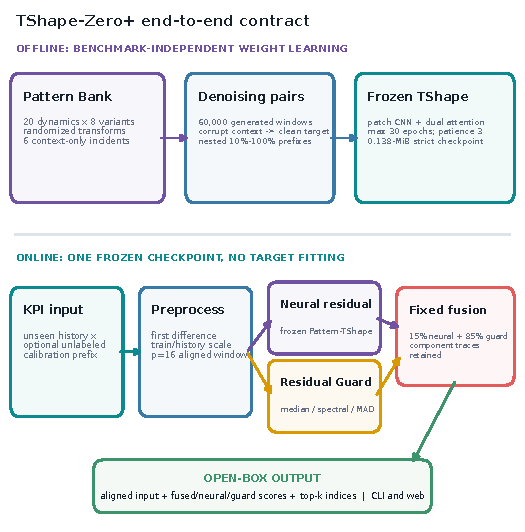
\includegraphics[width=\columnwidth]{figures/fig_framework_strict.pdf}
  \caption{End-to-end \method{} contract. Offline Pattern Bank generation produces one frozen TShape checkpoint without benchmark training. Online batch scoring applies documented preprocessing, computes neural and guard channels, fuses fixed weights, and returns aligned open-box evidence through CLI or web.}
  \label{fig:framework}
\end{figure}

Fig.~\ref{fig:framework} separates offline learning, target scoring, and product output. This separation makes each assumption reviewable: what enters the checkpoint, what uses unlabeled target context, how channels are normalized, and what an operator receives.

\subsection{Shared Preprocessing and Shape Channel}

For a history $x$, the scorer first applies a drop-first difference. In benchmark evaluation, min--max parameters are fitted on the series' unlabeled train history and applied to test; in the product, a user may provide a separate calibration history, otherwise the uploaded history supplies the affine scale. This target context changes no model weight. The product restores the differencing warm-up position with the minimum score so every returned index aligns with the raw upload.

We retain the original TShape architecture with $p=16$, four size-4 patches, a convolutional shape encoder, local/global attention, and squared next-value residuals. The Pattern-only channel is
\begin{equation}
 T_t^{\mathrm{PB}}=
 \left(z_t-f_{\theta^\star_{\mathrm{PB}}}(z_{t-p:t-1})\right)^2 ,
 \label{eq:pattern-score}
\end{equation}
where $z$ is the preprocessed target history and $\theta^\star_{\mathrm{PB}}$ is identical for all target datasets. The raw and normalized $T_t^{\mathrm{PB}}$ remain separately available in every product response.

\subsection{Pattern Bank Pretraining}

The Pattern Bank addresses missing temporal diversity without using benchmark samples. Its 20 \emph{normal} generators cover flat, polynomial, exponential, oscillatory, piecewise, stochastic, autoregressive, seasonal, growth, drift, and periodic-pulse dynamics. The taxonomy crosses four operational axes---level/trend, periodic structure, stochastic memory, and regime composition---while incident operators are kept orthogonal to the normal generator. It is a declared coverage prior, not a collection tuned against target labels. Eight randomized variants per family give 160 prototypes. A sampled prototype is transformed by amplitude, offset, reversal, slope, phase, and Gaussian noise. With probability 0.35, one of six incident operators injects a spike, dip, level shift, variance change, drift, or burst into the \emph{context only}. For clean prototype $u_{1:p+1}$, the denoising pair is
\begin{equation}
 \tilde w=u_{1:p}+\delta_{1:p},\qquad
 \tilde y=u_{p+1},
 \label{eq:pattern-pair}
\end{equation}
so the model learns continuation of the clean shape rather than reconstruction of the injected disturbance.

The release bank contains 60,000 generated windows. To test sample efficiency without changing motif composition, fraction $c\in\{0.1,0.2,\ldots,1.0\}$ uses the first $60{,}000c$ draws from one seeded stream. Thus the 10\% bank is a strict prefix of the 20\% bank, and so on; all levels contain all 20 generators in the same expected proportions. This design tests \emph{bank size}, not an arbitrary order of hand-added motif families. Every checkpoint trains with Adam ($10^{-3}$, batch 256) for at most 30 epochs and stops when training loss fails to improve by $10^{-5}$ for three consecutive epochs. The 100\% checkpoint is fixed before any target score is inspected and serves all six benchmarks.

\subsection{Residual Guard and Fusion}

For each target history, three label-free, no-training channels provide a reliability floor. $M_t$ is absolute deviation from the previous $p$-point rolling median. $S_t$ is spectral-residual saliency obtained by removing the smoothed log-amplitude spectrum. $D_t$ divides the rolling-median residual by a rolling MAD estimate. Let $N(\cdot)$ denote per-history min--max score normalization. The matched residual-only guard is
\begin{equation}
 G_t=\frac{0.55N(M_t)+0.25N(S_t)+0.05N(D_t)}{0.85}.
 \label{eq:guard}
\end{equation}
The release reserves a fixed 15\% neural budget and 85\% guard budget:
\begin{equation}
 \begin{aligned}
 s_t^{+} &=0.15N(T_t^{\mathrm{PB}})+0.85G_t \\
 &=0.15N(T_t^{\mathrm{PB}})+0.55N(M_t) \\
 &\quad+0.25N(S_t)+0.05N(D_t).
 \end{aligned}
 \label{eq:fusion}
\end{equation}
The weights are a predeclared reliability budget, not a benchmark-optimized solution. Weight sensitivity evaluates $\alpha\in\{0,0.05,0.10,0.15,0.25,0.50,1\}$, with the three guard weights renormalized inside $(1-\alpha)G_t$. Pairwise TShape+median and TShape+spectral variants test complementarity; a rank-normalized variant tests whether results depend on min--max magnitude. The matched comparison
\begin{equation}
 s_t^{+}-G_t=0.15\left(N(T_t^{\mathrm{PB}})-G_t\right)
 \label{eq:marginal}
\end{equation}
isolates the neural channel's marginal contribution after the exact guard is held fixed.

The present artifact scores complete historical sequences. Its normalization therefore supports offline triage and batch reliability analysis, not a claim of causal online thresholding. A streaming deployment would replace $N$ with a rolling source-calibrated transform; we leave that contract explicit instead of silently using future score extrema.

\subsection{Reviewable Product Contract}

The scorer accepts comma-, whitespace-, or newline-separated values. It returns the input trace, $s^+_t$, $T_t^{\mathrm{PB}}$, $G_t$, and top-$k$ indices. Metadata records the Pattern Bank version, size, seed, stopping rule, preprocessing, weights, and model hash. The web view invokes the same scorer as the CLI. Labels are optional retrospective case metadata and never required for scoring.

\section{Related Work}

\textbf{TSAD evaluation and reliability.}
Benchmark studies show that dataset quality, point adjustment, and aggregation can reverse anomaly-detector rankings~\cite{wu2021benchmarks,paparrizos2022volume,liu2024elephant}. TimeSeriesBench contributes industrial data, training schemas, and the EasyTSAD implementation used by the original TShape study~\cite{si2024timeseriesbench}. We preserve that protocol end to end and expose valid-series counts rather than combining incompatible metrics.

\textbf{Target-trained anomaly detectors.}
The original comparison spans classical local-discord and forecasting methods, reconstruction networks, frequency models, and attention architectures. Representative learned methods include USAD~\cite{audibert2020usad}, TranAD~\cite{tuli2022tranad}, Anomaly Transformer~\cite{xu2022anomaly}, TimesNet~\cite{wu2023timesnet}, OFA~\cite{zhou2023ofa}, FITS~\cite{zhou2024fits}, FCVAE~\cite{jiang2024fcvae}, and KAN-AD~\cite{li2025kanad}. Their published configurations are not uniformly packaged as frozen univariate scorers. We therefore distinguish official checkpoint executions from family adapters and source-adaptation diagnostics in every table.

\textbf{Foundation forecasting and zero-shot reuse.}
Timer, Chronos, TimesFM, Sundial, and Time-MoE broaden reusable time-series prediction~\cite{liu2024timer,ansari2024chronos,das2024timesfm,liu2025sundial,shi2024timemoe}. Our focal comparison executes three released checkpoints---Timer, Chronos, and Sundial---and converts chunk forecasts to squared residual scores without target fitting. Official TimeMoE-50M failed the study's practical ten-minute optional-checkpoint screen and is excluded rather than reported with its incomplete 240/834-series output; a separately marked family adapter remains in the ledger. Recent work targets zero-shot anomaly detection directly through pretrained predictors or cross-modal models~\cite{lan2025timercd,yang2026vetime}. Our contribution is complementary: it stress-tests and repairs a concrete TSAD artifact, and makes release maturity a first-class software reliability result.

\section{Evaluation}

\subsection{Research Questions}

The evaluation follows the dependencies of the released detector. \textbf{RQ1} asks whether one frozen \method{} checkpoint is effective relative to no-fit controls, official forecasting-foundation checkpoints, and the broader TShape baseline ledger. \textbf{RQ2} measures how Pattern Bank size changes optimization and EasyTSAD F1 on each target. \textbf{RQ3} isolates the failures repaired by the Residual Guard and the marginal value that remains attributable to TShape. \textbf{RQ4} examines the effectiveness--footprint tradeoff and the learned attention behavior on a real incident. All questions use the same two metrics defined in Section~II-A.

\subsection{Experimental Setup}

\begin{table}[t]
\caption{Full-coverage benchmark families. ``Ano.'' is the median anomalous-point ratio per series.}
\label{tab:data}
\centering
\scriptsize
\setlength{\tabcolsep}{3.2pt}
\begin{tabular}{lrrrr}
\toprule
Dataset & Series & Test points & Med. length & Med. ano. \\
\midrule
AIOPS & 29 & 3,073,556 & 131,795 & 1.269\% \\
NAB & 10 & 79,318 & 7,928 & 6.581\% \\
TODS & 15 & 75,000 & 5,000 & 5.360\% \\
UCR & 203 & 7,782,539 & 22,826 & 0.643\% \\
WSD & 210 & 3,829,537 & 18,236 & 0.310\% \\
Yahoo & 367 & 286,559 & 840 & 0.422\% \\
\midrule
Total & 834 & 15,126,509 & -- & -- \\
\bottomrule
\end{tabular}
\end{table}

\textbf{Datasets.}
Table~\ref{tab:data} contains 15.1 million observations from six distinct families. AIOPS comprises production KPIs from large Internet services, while WSD contains high-frequency Web-service KPIs; both directly represent software operations. NAB includes real streaming cloud, traffic, advertisement, and server-like signals~\cite{ahmad2017nab}. UCR contributes heterogeneous expert-labeled rare events, TODS contributes controlled anomaly variation, and Yahoo contributes real and synthetic Webscope streams. The original TShape study reports the first five; Yahoo is an artifact extension. The shared first-difference contract consumes one warm-up point per series, leaving 15,125,675 scored points. UCR, WSD, and Yahoo contain 2, 49, and 15 all-normal test series. They remain in coverage and resource totals but cannot define F1.

\textbf{Methods and access contracts.}
The public ledger contains 44 executable configurations and records whether each row is a no-fit control, released frozen checkpoint, strict synthetic-only checkpoint, source adaptation, family adapter, target-context diagnostic, or ablation. Table~\ref{tab:all-easytsad} omits the five residual controls and its Access column to keep the dense six-dataset comparison readable; their results remain available in the ledger and are analyzed explicitly in RQ3. Red/blue ranking in the table is restricted to released frozen foundation checkpoints and our strict synthetic-only checkpoints. This distinction remains essential: an adapter tests a scoring family under the common interface but is not represented as the original authors' checkpoint.

The residual controls are persistence, rolling mean, rolling median, spectral residual, and rolling MAD. The frozen-checkpoint group executes Chronos-Bolt-Tiny, Timer-base-84M, TimesFM-2.5-200M, and Sundial-base-128M directly; their preceding-context forecasts are converted to squared residual scores. Context/horizon pairs are 64/64, 384/96, 384/96, and 720/720. Official TimeMoE-50M exceeded the predeclared ten-minute optional-checkpoint screen and is not reported partially. A separately identified TimeMoE family adapter remains in the table. The ledger also retains every family represented in the original TShape comparison, including SubLOF, SAND, Matrix Profile, AR, LSTMAD, AE, EncDecAD, SRCNN, Anomaly Transformer, TFAD, TranAD, Donut, FCVAE, TimesNet, OFA, FITS, and KAN-AD.

\textbf{Execution and statistics.}
Every included method scores 834/834 series. All experiments use seed 20260704 on an 8-core Apple M3 with 16~GB unified memory. TShape uses PyTorch 2.0.0 with MPS, training batch 256, evaluation batch 2,048, and dense stride-one inference. The final Pattern checkpoint trains on all 60,000 generated windows with Adam, a maximum of 30 epochs, and patience-three early stopping. Labels are opened only after each score stream is frozen. For \method{} minus a comparator, the analysis unit is a series. We report mean paired difference and a 10,000-resample percentile bootstrap 95\% interval, together with wins, losses, ties, and an exact two-sided sign test in the artifact. These intervals measure cross-series heterogeneity under the fixed run; one seed does not establish training-seed stability.

The optimized metric adapter was checked against EasyTSAD 0.3.0.2 on 16 boundary traces and 200 randomized traces, including terminal events, tied scores, all-normal inputs, single-point events, and varying event lengths. \pfone{}, \efone{}, precision, recall, and selected thresholds matched exactly. Every result row exposes valid-series counts and coverage.

\subsection{RQ1: Overall Performance}

\begin{table*}[t]
\centering
\caption{Full-coverage non-residual comparison under one EasyTSAD protocol (Point-F1 / Event-F1). Among official frozen foundation checkpoints and strict synthetic-only TShape checkpoints, \textcolor{red}{red bold} and \textcolor{blue}{blue underlined} mark the best and second-best score per metric. Adapter, adaptation, diagnostic, and ablation provenance is retained in the public result ledger.}
\label{tab:all-easytsad}
\scriptsize
\setlength{\tabcolsep}{2.8pt}
\renewcommand{\arraystretch}{0.91}
\resizebox{\textwidth}{!}{%
\begin{tabular}{@{}llcccccc@{}}
\toprule
Family & Method & AIOPS & NAB & TODS & UCR & WSD & Yahoo \\
\midrule
Foundation & Chronos-Bolt-Tiny & 0.889 / 0.786 & 0.998 / 0.881 & 0.646 / 0.521 & 0.628 / 0.324 & 0.969 / 0.893 & \textcolor{blue}{\underline{0.762}} / \textcolor{blue}{\underline{0.739}} \\
 & Timer-base-84M & 0.886 / 0.781 & 0.990 / 0.862 & 0.752 / 0.615 & \textcolor{blue}{\underline{0.689}} / \textcolor{red}{\textbf{0.410}} & 0.963 / 0.890 & 0.731 / 0.699 \\
 & TimesFM-2.5-200M & \textcolor{red}{\textbf{0.896}} / \textcolor{red}{\textbf{0.800}} & 0.997 / 0.875 & \textcolor{red}{\textbf{0.818}} / \textcolor{red}{\textbf{0.688}} & \textcolor{red}{\textbf{0.705}} / \textcolor{blue}{\underline{0.399}} & \textcolor{red}{\textbf{0.971}} / \textcolor{red}{\textbf{0.901}} & 0.756 / 0.736 \\
 & Sundial-base-128M & 0.889 / \textcolor{blue}{\underline{0.792}} & 0.998 / 0.903 & 0.683 / 0.564 & 0.663 / 0.359 & \textcolor{blue}{\underline{0.971}} / \textcolor{blue}{\underline{0.894}} & 0.726 / 0.706 \\
 & TimerPatch & 0.836 / 0.624 & 0.998 / 0.890 & 0.625 / 0.435 & 0.696 / 0.431 & 0.899 / 0.727 & 0.528 / 0.497 \\
 & TimesFMTrend & 0.660 / 0.315 & 0.990 / 0.776 & 0.727 / 0.506 & 0.585 / 0.181 & 0.410 / 0.156 & 0.384 / 0.335 \\
 & SundialProb & 0.541 / 0.177 & 0.992 / 0.687 & 0.694 / 0.444 & 0.611 / 0.175 & 0.367 / 0.109 & 0.339 / 0.281 \\
 & TimeMixer & 0.789 / 0.578 & 0.996 / 0.858 & 0.781 / 0.586 & 0.604 / 0.222 & 0.747 / 0.474 & 0.467 / 0.426 \\
 & TimeMoE & 0.693 / 0.341 & 0.989 / 0.671 & 0.786 / 0.610 & 0.614 / 0.186 & 0.585 / 0.308 & 0.642 / 0.597 \\
\midrule
TSAD & ForecastResidual & 0.857 / 0.720 & 0.998 / 0.906 & 0.706 / 0.577 & 0.687 / 0.402 & 0.947 / 0.847 & 0.690 / 0.663 \\
 & OFA & 0.809 / 0.640 & 0.999 / 0.932 & 0.766 / 0.653 & 0.681 / 0.396 & 0.919 / 0.789 & 0.644 / 0.630 \\
 & FCVAE & 0.892 / 0.786 & 0.997 / 0.867 & 0.777 / 0.662 & 0.671 / 0.397 & 0.969 / 0.892 & 0.764 / 0.749 \\
 & TimesNet & 0.701 / 0.364 & 0.993 / 0.801 & 0.717 / 0.486 & 0.623 / 0.195 & 0.582 / 0.281 & 0.362 / 0.311 \\
 & KANAD & 0.770 / 0.538 & 0.998 / 0.887 & 0.580 / 0.391 & 0.684 / 0.413 & 0.861 / 0.692 & 0.445 / 0.414 \\
 & FITS & 0.683 / 0.452 & 0.991 / 0.740 & 0.788 / 0.691 & 0.614 / 0.365 & 0.765 / 0.629 & 0.512 / 0.487 \\
 & SubLOF & 0.851 / 0.662 & 0.997 / 0.806 & 0.701 / 0.572 & 0.640 / 0.333 & 0.911 / 0.759 & 0.563 / 0.507 \\
 & SAND & 0.900 / 0.790 & 0.998 / 0.895 & 0.773 / 0.676 & 0.672 / 0.390 & 0.975 / 0.895 & 0.766 / 0.752 \\
 & Matrix Profile & 0.626 / 0.284 & 0.985 / 0.735 & 0.497 / 0.282 & 0.561 / 0.327 & 0.806 / 0.541 & 0.302 / 0.248 \\
 & AR & 0.608 / 0.218 & 0.991 / 0.629 & 0.654 / 0.347 & 0.606 / 0.180 & 0.371 / 0.124 & 0.271 / 0.213 \\
 & LSTMAD & 0.894 / 0.788 & 0.998 / 0.884 & 0.763 / 0.691 & 0.658 / 0.397 & 0.975 / 0.896 & 0.740 / 0.712 \\
 & AE & 0.895 / 0.798 & 0.998 / 0.881 & 0.810 / 0.743 & 0.641 / 0.386 & 0.972 / 0.897 & 0.761 / 0.746 \\
 & EncDecAD & 0.662 / 0.433 & 0.996 / 0.829 & 0.566 / 0.325 & 0.599 / 0.187 & 0.538 / 0.384 & 0.302 / 0.267 \\
 & SRCNN & 0.896 / 0.684 & 0.993 / 0.678 & 0.729 / 0.558 & 0.739 / 0.354 & 0.918 / 0.668 & 0.624 / 0.594 \\
 & TFAD & 0.896 / 0.748 & 0.998 / 0.886 & 0.774 / 0.659 & 0.691 / 0.409 & 0.963 / 0.852 & 0.767 / 0.752 \\
 & Donut & 0.882 / 0.764 & 0.998 / 0.882 & 0.789 / 0.702 & 0.652 / 0.387 & 0.958 / 0.878 & 0.753 / 0.735 \\
 & USAD & 0.682 / 0.304 & 0.995 / 0.820 & 0.486 / 0.254 & 0.533 / 0.330 & 0.813 / 0.550 & 0.198 / 0.149 \\
 & TranAD & 0.692 / 0.349 & 0.990 / 0.745 & 0.448 / 0.233 & 0.514 / 0.333 & 0.738 / 0.416 & 0.379 / 0.357 \\
 & Anomaly Transformer & 0.636 / 0.280 & 0.993 / 0.814 & 0.441 / 0.247 & 0.502 / 0.306 & 0.730 / 0.401 & 0.220 / 0.166 \\
\midrule
TShape & Pattern-only TShape-Zero & 0.867 / 0.758 & \textcolor{red}{\textbf{0.999}} / \textcolor{red}{\textbf{0.926}} & 0.694 / 0.622 & 0.637 / 0.380 & 0.951 / 0.869 & 0.666 / 0.651 \\
 & \textbf{TShape-Zero+$^{\star}$} & \textcolor{blue}{\underline{0.895}} / 0.769 & \textcolor{blue}{\underline{0.999}} / \textcolor{blue}{\underline{0.918}} & \textcolor{blue}{\underline{0.766}} / \textcolor{blue}{\underline{0.673}} & 0.669 / 0.396 & 0.967 / 0.873 & \textcolor{red}{\textbf{0.779}} / \textcolor{red}{\textbf{0.769}} \\
 & LODO TShape adaptation & 0.871 / 0.767 & 0.998 / 0.906 & 0.671 / 0.597 & 0.629 / 0.377 & 0.958 / 0.879 & 0.723 / 0.689 \\
 & PB Hybrid & 0.869 / 0.764 & 0.999 / 0.926 & 0.680 / 0.599 & 0.633 / 0.376 & 0.961 / 0.882 & 0.747 / 0.737 \\
 & PB Source-CV & 0.886 / 0.782 & 0.998 / 0.879 & 0.741 / 0.674 & 0.645 / 0.402 & 0.964 / 0.888 & 0.770 / 0.759 \\
 & Fixed 0.15 Fusion & 0.895 / 0.769 & 0.998 / 0.911 & 0.765 / 0.676 & 0.669 / 0.399 & 0.968 / 0.875 & 0.772 / 0.762 \\
 & PB100+Guard & 0.896 / 0.761 & 0.999 / 0.920 & 0.772 / 0.673 & 0.674 / 0.406 & 0.966 / 0.870 & 0.769 / 0.757 \\
 & LODO Zero+ diagnostic & 0.895 / 0.760 & 0.998 / 0.907 & 0.774 / 0.671 & 0.677 / 0.406 & 0.966 / 0.869 & 0.769 / 0.756 \\
 & Target-Context Diagnostic & 0.885 / 0.784 & 0.998 / 0.883 & 0.669 / 0.588 & 0.625 / 0.363 & 0.963 / 0.885 & 0.662 / 0.653 \\
 & Residual-Only Guard & 0.895 / 0.760 & 0.998 / 0.902 & 0.773 / 0.669 & 0.676 / 0.405 & 0.964 / 0.864 & 0.769 / 0.755 \\
 & Direct+Guard & 0.894 / 0.768 & 0.999 / 0.920 & 0.765 / 0.677 & 0.672 / 0.403 & 0.968 / 0.872 & 0.761 / 0.738 \\
\bottomrule
\end{tabular}}
\renewcommand{\arraystretch}{1.0}
\end{table*}


Table~\ref{tab:all-easytsad} is the primary non-residual result. It keeps every completed foundation, TSAD, and TShape configuration and all six targets visible, while access provenance remains machine-readable in the public ledger. The red and blue values answer a narrow, reproducible question: among official frozen checkpoints and strict synthetic-only TShape checkpoints, which score streams are strongest under the common EasyTSAD protocol? Adapter and diagnostic rows broaden the empirical landscape but cannot win that ranking.

\begin{figure}[t]
  \centering
  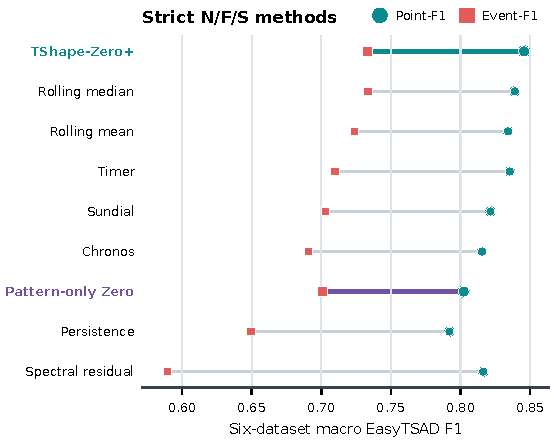
\includegraphics[width=\columnwidth]{figures/fig_strict_overall.pdf}
  \caption{Macro performance of directly deployable no-fit, frozen, and strict synthetic-only methods. Each segment connects a method's \efone{} (square) and \pfone{} (circle). Table~\ref{tab:all-easytsad} reports the non-residual per-dataset results; the public ledger retains access status for every method.}
  \label{fig:overall}
\end{figure}

Fig.~\ref{fig:overall} makes the central comparison readable without hiding the long table. Pattern-only TShape-Zero reaches \PatternMacroPoint{}/\PatternMacroEvent{} macro \pfone{}/\efone{}. Adding the guard raises the result to \FinalMacroPoint{}/\FinalMacroEvent{}, a gain of 0.044/0.032. TimesFM is the strongest official checkpoint on macro \pfone{} at 0.857 and obtains 0.733 macro \efone{}; \method{} is 0.012 lower on \pfone{} and effectively tied at the reported three-decimal \efone{} precision. Rolling median remains a serious deployment control at 0.839/0.734. Thus, the result supports a compact and inspectable TShape upgrade, not universal superiority.

The per-dataset cells expose complementary regimes. Among the ranked frozen/strict checkpoints, \method{} is strongest on Yahoo for both metrics and second on AIOPS and TODS \pfone{}, while the Pattern-only checkpoint is strongest on NAB. TimesFM leads AIOPS, TODS, and WSD and leads UCR \pfone{}; Timer leads UCR \efone{}. Some adapter rows obtain larger individual cells under different packaging or adaptation contracts, which is why their provenance remains explicit in the public ledger rather than being conflated with official frozen-checkpoint evidence. This heterogeneity is precisely why an out-of-the-box product must retain channel evidence and why average-only claims would be unsafe.

\textbf{Answer to RQ1.}
One strict \method{} checkpoint provides full six-dataset coverage and is competitive with checkpoints thousands of times larger. It substantially repairs Pattern-only TShape, but strong foundation and residual controls still win particular targets and metrics.

\subsection{RQ2: Pattern Bank Effectiveness}

\begin{figure}[t]
  \centering
  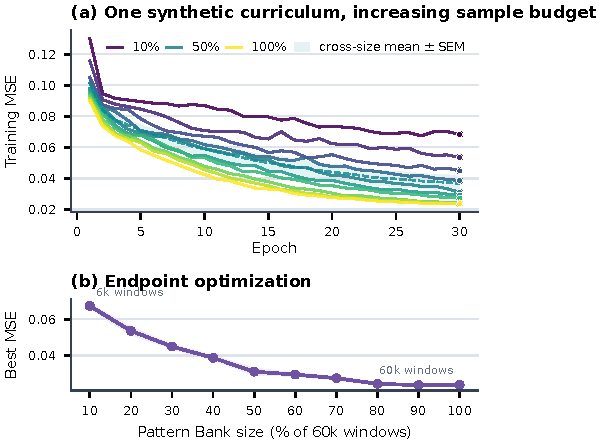
\includegraphics[width=\columnwidth]{figures/fig_strict_pattern_training.pdf}
  \caption{Pattern Bank optimization from 10\% to 100\%. (a) Training trajectories and their cross-size envelope. (b) Best training MSE against the nested number of generated windows. Every size uses the same generator mixture and seed.}
  \label{fig:pattern-training}
\end{figure}

\begin{figure}[t]
  \centering
  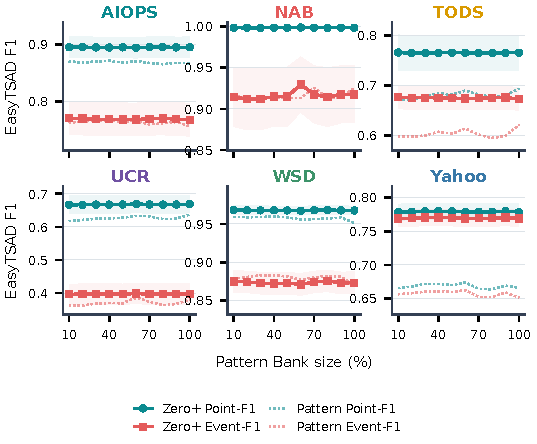
\includegraphics[width=\columnwidth]{figures/fig_strict_pattern_effect.pdf}
  \caption{Pattern Bank size sweep on all six datasets, arranged as two rows of three panels. Dotted curves are the neural Pattern-only channel; solid curves are the same checkpoints after the fixed Residual Guard. Every point is a full-series \pfone{} or \efone{} evaluation; labeled panel-specific ranges expose within-target change without implying cross-panel scale equality.}
  \label{fig:pattern-effect}
\end{figure}

The size sweep uses strict nested prefixes of one generated stream: 10\% contains 6,000 windows and each step adds 6,000 until the 60,000-window bank is complete. Generator identities, random seed, incident rate, optimizer, maximum epochs, and stopping rule remain fixed. Consequently, Fig.~\ref{fig:pattern-training} measures additional generated evidence rather than an order-dependent addition of hand-selected pattern families.

Training loss and target F1 answer different questions. More generated windows constrain continuation on the Pattern Bank, so optimization should improve or saturate. An unseen benchmark, however, is never consulted when choosing bank size; its F1 may fluctuate because additional synthetic variation can help one target and dilute another. Fig.~\ref{fig:pattern-effect} therefore reports every measured endpoint rather than smoothing the curve into artificial monotonicity. The 100\% checkpoint is the release model because it realizes the predeclared full-diversity curriculum, not because target labels selected a favorable fraction.

The measured curves make this boundary concrete. Best training MSE falls from 0.0674 with 6,000 windows to 0.0237 with 60,000, a 64.8\% reduction, and the slope visibly flattens after 48,000 windows. Across targets, Pattern-only macro \pfone{}/\efone{} starts at 0.797/0.696, reaches 0.804/0.703 at 60\%, and finishes at 0.802/0.701. The additional bank evidence is clearest on TODS (0.673 to 0.694 \pfone{}) and UCR (0.617 to 0.637), while already saturated or mismatched targets show smaller reversals. After the fixed guard, all ten checkpoints lie in the narrow 0.845--0.846 \pfone{} and 0.733--0.735 \efone{} bands. Thus the bank improves the learned synthetic objective and selected transfer regimes, while the guard converts target-specific fluctuations into a stable release envelope.

The six panels also separate learning from fallback behavior. A movement in a dotted curve is attributable to the checkpoint. A smaller movement in the corresponding solid curve means that the fixed guard absorbs neural instability; a larger movement means that newly learned shape evidence complements the guard. This distinction prevents the Pattern Bank claim from borrowing gains produced by residual channels.

\textbf{Answer to RQ2.}
The Pattern Bank supplies measurable zero-shot shape evidence under a benchmark-independent training contract. Increasing generated coverage sharply improves and then saturates the training objective, but target F1 is not guaranteed to be monotone. The fixed guard reduces the operational cost of that residual transfer variance; the 100\% release is selected by coverage policy, not target-label performance.

\subsection{RQ3: Residual Guard Effectiveness}

\begin{figure}[t]
  \centering
  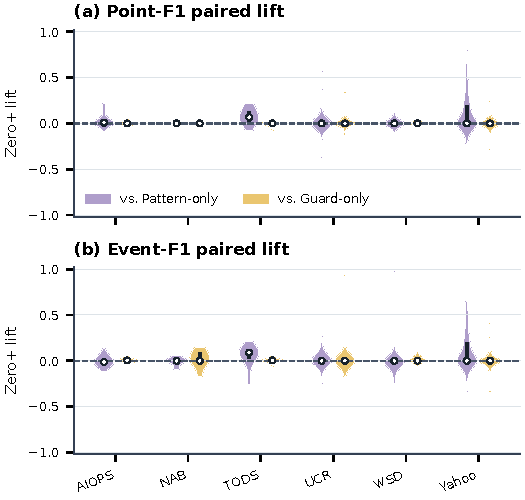
\includegraphics[width=\columnwidth]{figures/fig_strict_guard_violin.pdf}
  \caption{Paired series-level lift of \method{} over Pattern-only TShape (purple) and over the exactly matched residual-only guard (gold). Violin density, interquartile bar, and median expose both average repair and harmed series.}
  \label{fig:guard-violin}
\end{figure}

\begin{figure}[t]
  \centering
  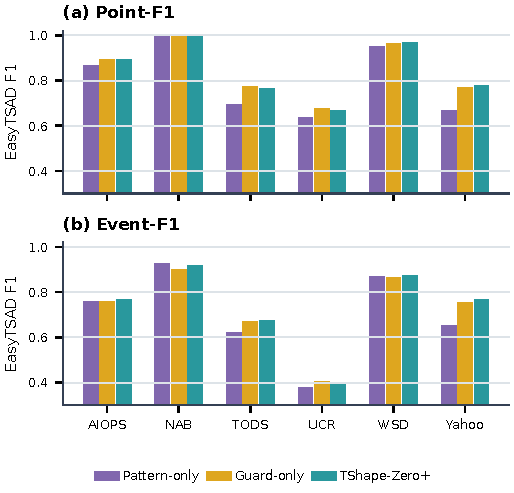
\includegraphics[width=\columnwidth]{figures/fig_strict_guard_bars.pdf}
  \caption{Dataset-level decomposition for Pattern-only, guard-only, and final \method{}. The neural comparison isolates repair; the matched-guard comparison isolates TShape's marginal contribution.}
  \label{fig:guard-bars}
\end{figure}

Figs.~\ref{fig:guard-violin} and~\ref{fig:guard-bars} separate algorithmic contribution from engineering protection. Relative to Pattern-only TShape, final fusion improves macro \pfone{} by 0.044 and macro \efone{} by 0.032. Point-F1 gains are positive with bootstrap intervals above zero on AIOPS, TODS, UCR, WSD, and Yahoo; Yahoo gains 0.113/0.118 in paired mean \pfone{}/\efone{}. NAB is already saturated and its small Event-F1 change is negative.

The stricter comparator is the guard itself. Guard-only obtains \GuardMacroPoint{}/\GuardMacroEvent{}, versus \FinalMacroPoint{}/\FinalMacroEvent{} for final fusion. Their macro \pfone{} values are effectively equal, while TShape adds 0.007 macro \efone{}. At series level, the Event-F1 intervals are positive on AIOPS, WSD, and Yahoo; UCR remains a failure boundary. This is a bounded but nonzero neural contribution: the guard supplies most of the reliability floor, while learned repeated-shape evidence improves selected event regimes.

\begin{table}[t]
\caption{Paired series-level repair effects. Cells are mean difference [bootstrap 95\% interval]. PB: strict Pattern-only TShape-Zero; G: matched residual-only guard.}
\label{tab:paired-effects}
\centering
\scriptsize
\setlength{\tabcolsep}{2.3pt}
\resizebox{\columnwidth}{!}{%
\begin{tabular}{lrrrr}
\toprule
Dataset & $\Delta$Point vs. PB & $\Delta$Event vs. PB & $\Delta$Point vs. G & $\Delta$Event vs. G \\
\midrule
AIOPS & +0.028 [+0.006,+0.053] & +0.011 [-0.019,+0.047] & +0.000 [-0.007,+0.007] & +0.009 [+0.002,+0.017] \\
NAB & -0.000 [-0.001,+0.000] & -0.008 [-0.035,+0.016] & +0.000 [-0.001,+0.002] & +0.016 [-0.040,+0.066] \\
TODS & +0.072 [+0.030,+0.115] & +0.052 [-0.009,+0.104] & -0.008 [-0.022,+0.002] & +0.004 [-0.010,+0.015] \\
UCR & +0.032 [+0.012,+0.053] & +0.016 [-0.006,+0.041] & -0.008 [-0.018,+0.003] & -0.008 [-0.033,+0.017] \\
WSD & +0.016 [+0.004,+0.033] & +0.005 [-0.016,+0.027] & +0.003 [+0.000,+0.006] & +0.009 [+0.002,+0.016] \\
Yahoo & +0.113 [+0.090,+0.136] & +0.118 [+0.095,+0.142] & +0.010 [-0.000,+0.020] & +0.015 [+0.003,+0.026] \\
\bottomrule
\end{tabular}}
\end{table}


\begin{figure}[t]
  \centering
  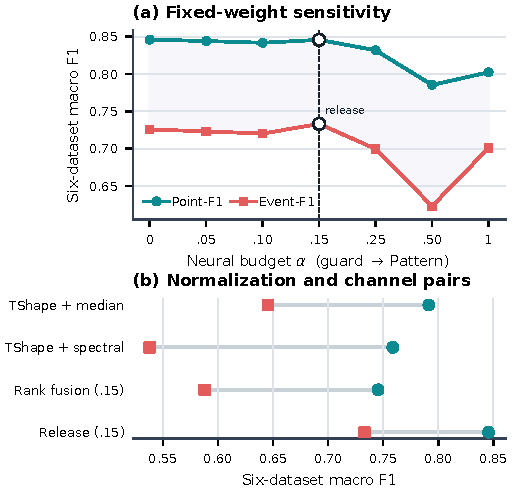
\includegraphics[width=\columnwidth]{figures/fig_strict_guard_ablation.pdf}
  \caption{Residual Guard ablations over six-dataset macro \pfone{} and \efone{}. The sweep varies neural budget $\alpha$, score normalization, and pairwise evidence channels while holding the strict Pattern checkpoint fixed.}
  \label{fig:guard-ablation}
\end{figure}

The ablation in Fig.~\ref{fig:guard-ablation} tests whether Eq.~\eqref{eq:fusion} is merely a renamed residual ensemble. The endpoints $\alpha=0$ and $\alpha=1$ are guard-only and Pattern-only. The release obtains \FinalMacroPoint{}/\FinalMacroEvent{} at $\alpha=0.15$; guard-only obtains \GuardMacroPoint{}/\GuardMacroEvent{}. Thus the guard is marginally higher in macro \pfone{}, while 0.15 is higher in macro \efone{}. Raising the neural budget to 0.50 reduces the scores to 0.785/0.623, showing why residual-first weighting is necessary. TShape+median and TShape+spectral reach only 0.792/0.645 and 0.759/0.538, so no single guard component explains the final result. Rank-normalized 0.15 fusion reaches 0.745/0.588, confirming that the documented min--max score contract is consequential. The release keeps $\alpha=0.15$ as a conservative, predeclared reliability budget; we do not relabel it as universally target-optimal.

\begin{figure}[t]
  \centering
  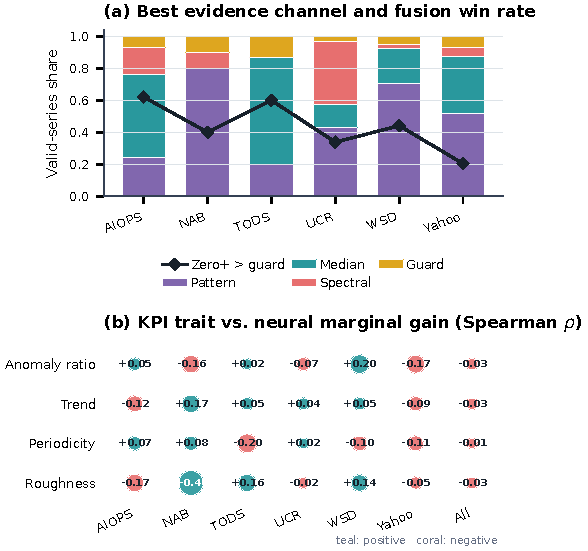
\includegraphics[width=\columnwidth]{figures/fig_strict_channel_attribution.pdf}
  \caption{EasyTSAD channel attribution over paired valid series. (a) Stacked bars identify the strongest individual evidence channel; diamonds show how often final fusion beats the exactly matched guard. (b) Bubble size and color encode the Spearman association between four unlabeled KPI traits and final fusion gain. This is a diagnostic, not a target-trained gate.}
  \label{fig:channel-attribution}
\end{figure}

Fig.~\ref{fig:channel-attribution} asks a stricter question than a favorable case study: can one explain when the neural channel adds value? Panel (a) compares Pattern-only TShape with median, spectral, and combined-guard evidence on every paired valid series, then reports the final fusion win rate against that same guard. Panel (b) relates the paired mean of Point-F1 and Event-F1 gains to anomaly ratio, trend, periodicity, and roughness. The traits are computed only after scores are frozen and are never used for checkpoint or weight selection. Their associations are descriptive rather than a learned target gate; weak or conflicting cells are themselves evidence that channel attribution should be returned to the operator instead of being replaced by an opaque universal routing rule.

\textbf{Answer to RQ3.}
The Residual Guard is responsible for most average robustness, and the paper states that fact directly. TShape remains useful where repeated local/global shape evidence improves event ranking beyond the matched guard, especially on AIOPS, WSD, and Yahoo; it is not indispensable on every KPI.

\subsection{RQ4: Effectiveness, Footprint, and Learned Behavior}

\begin{figure}[t]
  \centering
  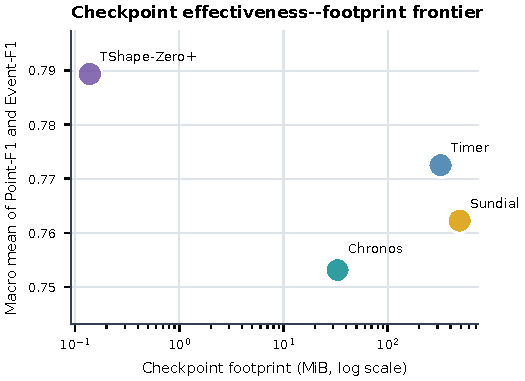
\includegraphics[width=\columnwidth]{figures/fig_strict_effectiveness_bubble.pdf}
  \caption{Effectiveness--distribution frontier for strict frozen checkpoints. Position is checkpoint footprint versus mean macro F1; bubble area encodes macro \efone{}. Upper left is preferable.}
  \label{fig:effectiveness}
\end{figure}

Fig.~\ref{fig:effectiveness} combines effectiveness with release cost. The \method{} checkpoint is 0.138 MiB, compared with 33.0 MiB for Chronos, 321.0 MiB for Timer, 489.6 MiB for Sundial, and 882.3 MiB for TimesFM. TimesFM's macro advantage is 0.012 \pfone{} and less than 0.001 \efone{}, while its distributed checkpoint is over 6,000 times larger. The final Pattern model trains in 128 seconds; dense stride-one inference over all 834 series and 15.1 million aligned points takes 291 seconds on the study MPS device. Footprint is not latency, but it directly affects artifact transfer, cold start, versioning, and edge placement. Runtime metadata remain available separately so the bubble plot does not pretend that heterogeneous foundation-model hardware timings are architecture-only effects.

\begin{figure}[t]
  \centering
  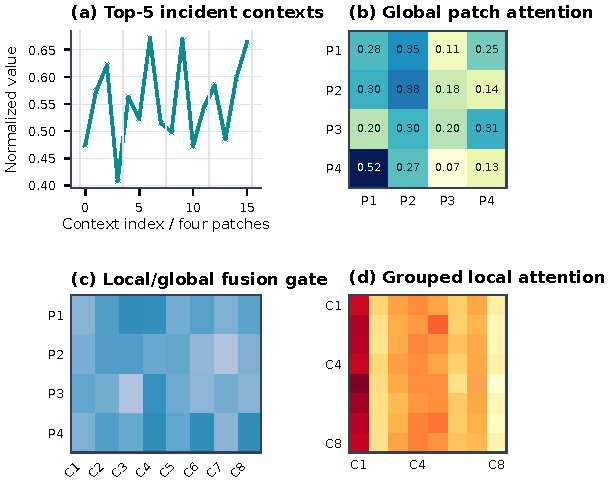
\includegraphics[width=\columnwidth]{figures/fig_strict_attention.pdf}
  \caption{Mechanism trace for the frozen checkpoint on top-ranked points from the real deployment case: incident contexts, global patch attention, local/global fusion gate, and grouped local attention. Attention is descriptive evidence, not a causal explanation.}
  \label{fig:attention}
\end{figure}

Fig.~\ref{fig:attention} verifies that the released neural channel is active rather than a dead weight in the residual ensemble. On the top-ranked incident contexts, global attention connects nonadjacent patches while the fusion gate varies across patches and channels. The local map emphasizes repeated within-patch structure. These traces establish input-dependent execution and support debugging; they do not prove that an attention coefficient caused a correct alarm.

\textbf{Answer to RQ4.}
\method{} occupies a favorable compact-checkpoint region and exposes internal and residual evidence through one scorer. Its efficiency claim is distribution footprint and full-series executability, not an unsupported universal latency claim.

\subsection{Threats to Validity}

\textbf{Construct validity.}
Point adjustment can reward long events~\cite{kim2022rigorous}. We use it because the original TShape claim uses EasyTSAD, pair it with logarithmic event weighting, and apply the exact same implementation to every score stream. Both metrics select thresholds with labels and therefore evaluate score separability, not an online alarm policy.

\textbf{Internal validity.}
One fixed seed makes the full sweep reproducible and computationally tractable but cannot quantify optimizer-seed variance. Series-level bootstrap intervals quantify target heterogeneity only. Official foundation checkpoints and no-fit controls are ranked separately from adapters, source adaptation, and target-context diagnostics. The Pattern Bank checkpoint metadata states that no benchmark values or labels enter weight fitting.

\textbf{Baseline validity.}
Four foundation rows use released checkpoints directly. Many anomaly families lack an equivalent frozen univariate interface; their X rows are executable family adapters, not claims of official reproduction. Unknown overlap between public benchmarks and foundation pretraining corpora may advantage those checkpoints. TimeMoE is omitted under the predeclared runtime rule rather than completed on a biased subset.

\textbf{External and deployment validity.}
The six families span industrial Internet-service KPIs, Web-service monitoring, public cloud streams, controlled anomalies, and rare-event archives, but remain univariate historical benchmarks. Proprietary multivariate and causal streaming settings may differ. Per-history score normalization uses the complete batch; online deployment requires a rolling or source-calibrated transform. The web case is illustrative and selected after the aggregate protocol was frozen, so it is not used as independent effectiveness evidence.


\section{Deployment}

\subsection{Versioned Product Surface}

The public artifact at \url{https://github.com/CSTCloudOps/TShape-Zero} packages the strict checkpoint, shared scorer, CLI, and web interface as one versioned product. The checkpoint metadata records Pattern Bank version and size, seed, preprocessing, stopping rule, fusion weights, and SHA256 digest. A verification ledger maps every reported cell to method status, valid-series count, coverage, and metric implementation. Dataset licenses are respected through acquisition instructions and a checksum manifest rather than silent redistribution.

\begin{figure}[t]
  \centering
  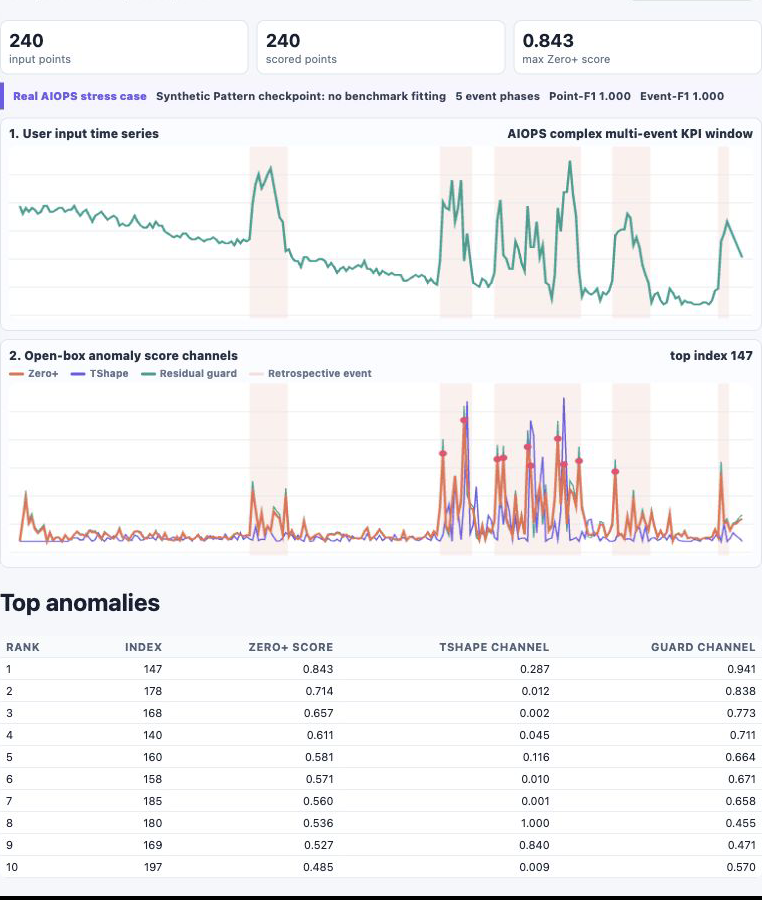
\includegraphics[width=\columnwidth]{figures/fig_product_strict_panel.png}
  \caption{Released web scorer on a complex real 240-point AIOPS incident window. The interface returns the aligned KPI trace, fused/neural/guard scores, and ranked suspicious points from the same scorer used by the CLI.}
  \label{fig:product}
\end{figure}

Fig.~\ref{fig:product} shows the product path on a real AIOPS window with baseline drift and five anomaly phases, including bursts, plateaus, partial recoveries, and renewed excursions. The user pastes or uploads history and may optionally provide a separate unlabeled calibration prefix. The service validates numeric input, applies the documented difference-and-scale contract, runs the frozen 0.138-MiB checkpoint and three guard channels, restores raw-index alignment, and returns two linked plots plus a top-$k$ table. No target label, gradient step, or target-specific checkpoint selection occurs.

For this 240-point case, \method{} obtains retrospective local \pfone{} 1.000 and \efone{} 1.000, and all ten highest-scored points lie inside labeled incident phases. The case is intentionally demanding rather than a single isolated spike. It was selected for interface demonstration only after the model and aggregate evaluation were frozen; its values, labels, channel scores, and selection rule are included so reviewers can reproduce the screenshot and recognize that it is not a held-out statistical result.

The deployment contract exposes failure rather than hiding it. The default response returns continuous scores and component attribution, not an EasyTSAD oracle threshold. Invalid or too-short histories fail with an actionable message. The reviewer workflow verifies metric conformance without data, scores a bundled smoke trace, regenerates the case, and then optionally executes the full 834-series tier. CLI and web requests share one scoring function, so interface drift cannot silently change the paper result. The current release is a batch historical scorer; causal streaming normalization and automated paging policy are explicit future contracts.

\subsection{Executable Deployment Contract}

Table~\ref{tab:deployment-contract} makes the product boundary testable. A request contains a numeric univariate history and may contain a separate unlabeled calibration prefix. The service rejects malformed values and histories shorter than the model context. A successful response has the same raw index space as the upload and contains the fused score, neural score, guard score, ranked indices, and immutable model metadata. The one-point differencing warm-up is restored as a non-alarming pad rather than silently shifting incident locations. This alignment check is important in operations, where an off-by-one alert can associate an anomaly with the wrong deployment or log window.

\begin{table}[t]
\caption{Executable product and reviewer contract.}
\label{tab:deployment-contract}
\centering
\scriptsize
\setlength{\tabcolsep}{3.0pt}
\begin{tabular}{>{\raggedright\arraybackslash}p{0.20\columnwidth}>{\raggedright\arraybackslash}p{0.39\columnwidth}>{\raggedright\arraybackslash}p{0.31\columnwidth}}
\toprule
Contract & Shipped behavior & Verification assertion \\
\midrule
Checkpoint & 145,215 bytes; immutable metadata and digest & Hash and strict-training flags match \\
Input & Numeric history; optional unlabeled calibration prefix & Malformed and short inputs fail \\
Alignment & Warm-up pad restores raw upload indices & Output length equals input length \\
Evidence & Fused, neural, guard, and ranked suspicious points & Fixed fusion recomputes exactly \\
Labels & Never accepted by the scoring path & Case labels are overlay-only \\
Coverage & One checkpoint for all six benchmark families & Ledger contains 834/834 series \\
\bottomrule
\end{tabular}
\end{table}

The open-box response also supports an operational decision rule without pretending to solve alarm policy. When neural and guard channels agree at a top-ranked point, the operator receives two independent forms of evidence. A guard-dominated point indicates a sharp level, spectral, or robust-deviation change that the learned channel may not recognize; this is the intended reliability-floor behavior. A neural-dominated point indicates a shape-continuation violation not fully explained by the residual controls. Repeated disagreement is not hidden by the fused score: it is a signal to inspect preprocessing, provide a representative unlabeled calibration history, or fall back to target training before connecting the detector to paging.

\subsection{Reviewer Workflow and Release Tiers}

The release provides three verification tiers. The no-data tier checks the checkpoint digest, score formula, output alignment, deterministic smoke trace, and exact EasyTSAD adapter on boundary and randomized inputs. The case tier regenerates Fig.~\ref{fig:product} from the bundled 240-point history and verifies the displayed top-$k$ ordering and component scores. The full tier acquires each dataset from its documented source, verifies checksums, executes all 834 series, and rebuilds the 44-by-6 ledger, paired intervals, tables, and figures. Each tier emits a machine-readable report, so a reviewer can distinguish ``the interface runs'' from ``the complete empirical claim was reproduced.''

For an SRE team, the recommended present use is historical triage or shadow deployment. The product immediately ranks suspicious regions and exposes why they were ranked; the team then chooses a top-$k$, source-calibrated, or policy-specific alarm threshold using its own false-alert budget. If storage and cold-start cost are secondary, Table~\ref{tab:all-easytsad} shows that a large forecasting foundation checkpoint may be preferable on some KPIs. If a stable target history and retraining budget exist, target-trained TShape remains valid. The release therefore turns empirical heterogeneity into a concrete choice among compact out-of-the-box triage, a larger foundation checkpoint, and target-specific training.


\section{Conclusion}

We preserve TShape's original target-trained claim and turn the stronger out-of-the-box requirement into a constructive artifact repair. \method{} trains one compact TShape checkpoint on a benchmark-independent generated Pattern Bank, protects shifted KPIs with an inspectable Residual Guard, and ships preprocessing, scoring, verification, CLI, and web contracts together. Under one EasyTSAD protocol, the frozen checkpoint scores all 834 series and reaches macro \pfone{}/\efone{} of \FinalMacroPoint{}/\FinalMacroEvent{}. The guard supplies most average robustness; the neural channel adds bounded event-level value on identifiable regimes, and the paper exposes both facts through matched ablations. Strong residual and foundation checkpoints prevent a universal-SOTA claim, while the 0.138-MiB footprint and reproducible deployment case establish practical release value. The broader reliability lesson is concrete: reusable anomaly detection requires not only model weights, but also data-access provenance, transparent fallback behavior, metric-compatible evidence, coverage, and an executable product contract.

\clearpage
\bibliographystyle{IEEEtran}
\bibliography{references}

\end{document}
